\subsubsection{Motherboard}
Für die Unterbringung der Elektronik in der Maschine dient ein Brett
als Grundlage für ein Motherboard. Dieses trägt den Grossteil der
Elektronik auf sich. Zentral gelegen wird es als Ausgangspunkt für
jegliche Verdrahtung und Verkabelung zwischen Platinen, Komponenten und der
Energieversorgung genutzt. Lediglich der BLDC-Regler, die Endschalter 
als auch das DC-Treiberboard sind anderweitig im Turm untergebracht.
Die Abbildung \ref{fig:motherboard_pcb} zeigt den Aufbau des Motherboards
und benennt die einzelnen Komponentengruppen.

%\begin{figure}[h!]
%	\centering
%	\begin{subfigure}[b]{0.48\textwidth}
%		\centering
%		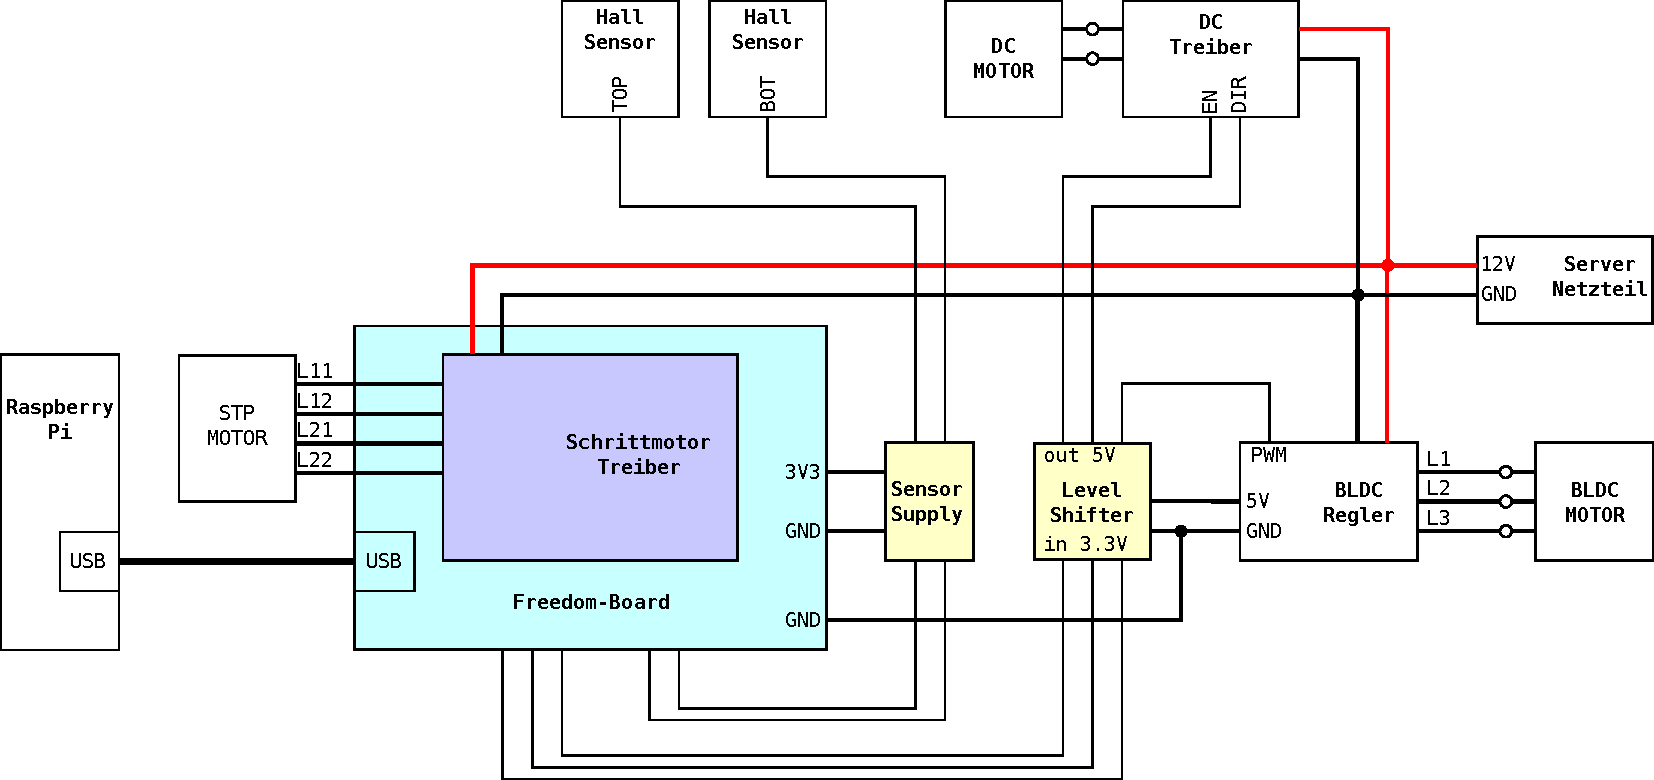
\includegraphics[width=1\textwidth]{../../fig/et/motherboard.png}
%		\caption{Motherboard aus der Seitenansicht}
%	\end{subfigure}
%	\begin{subfigure}[b]{0.48\textwidth}
%		\centering
%		\includegraphics[angle=90, width=1\textwidth]{../../fig/et/motherboard_02.png}
%		\caption{Motherboard aus der Vogelperspektive}
%	\end{subfigure}
%	\caption{Motherboard}
%\end{figure}

\begin{figure}[h!]
	\centering
	\includegraphics[width=0.7\textwidth]{../../fig/et/motherboard_ov.pdf}
	\caption{Motherboard in der Übersicht}
	\label{fig:motherboard_pcb}
\end{figure}

%\begin{figure}[h!]
%	\centering
%	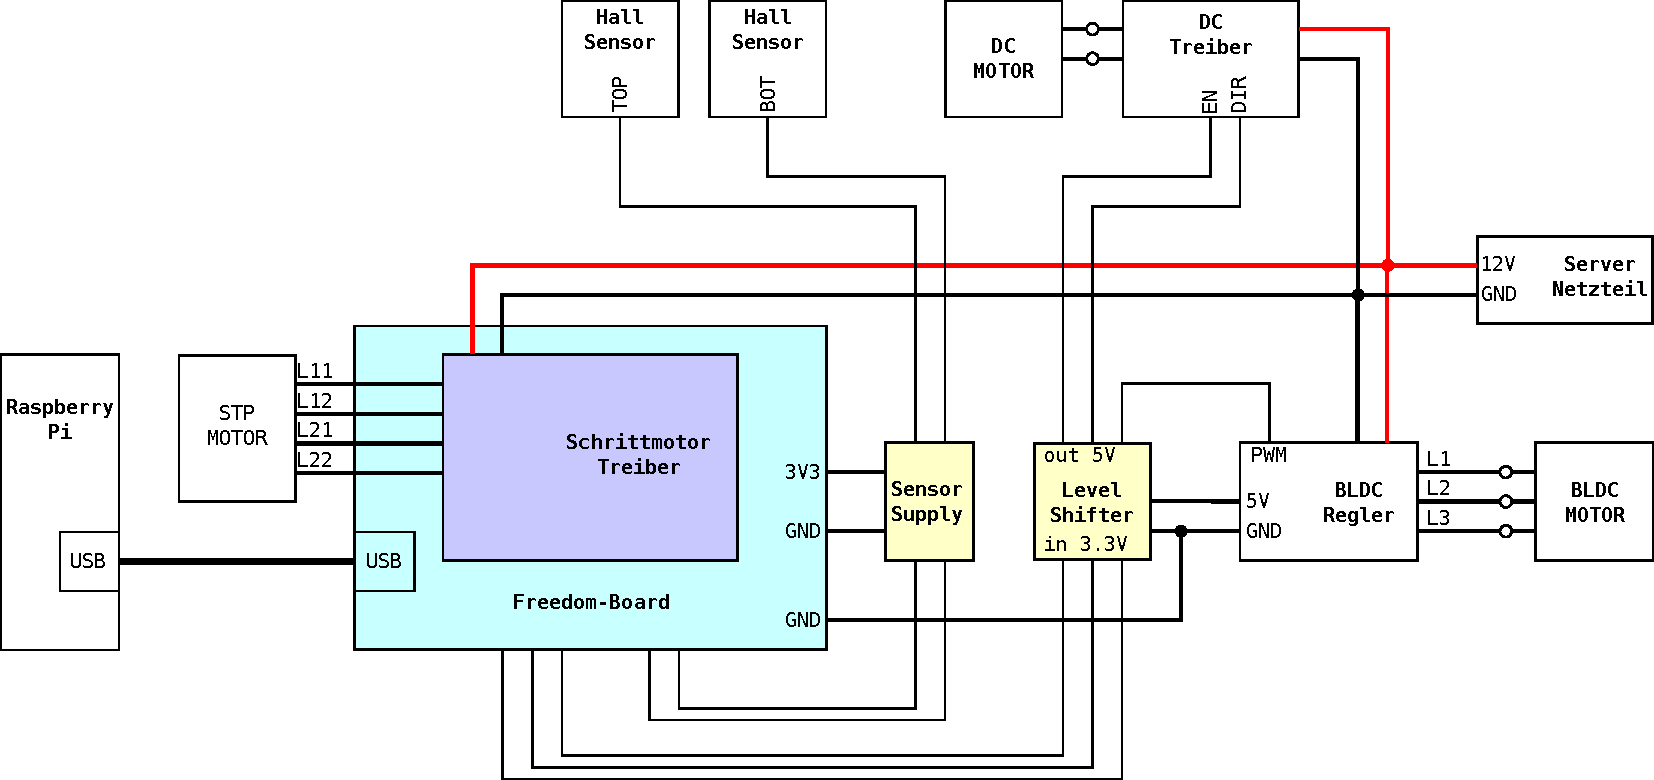
\includegraphics[width=0.8\textwidth]{../../fig/et/motherboard.pdf}
%	\caption{Motherboard im Blockschaltbild}
%	\label{fig:motherboard_block}
%\end{figure}
